\documentclass[11pt]{article}

% Users of the {thebibliography} environment or BibTeX should use the
% scicite.sty package, downloadable from *Science* at
% www.sciencmag.org/misc/con-info.shtml .  This package should properly
% format in-text reference calls and reference-list numbers.
\usepackage{epsfig}
\usepackage{geometry}
\geometry{letterpaper}
\usepackage{graphicx}
\usepackage{amssymb}
\usepackage{epstopdf}
%\DeclareGraphicsRule{.tif}{png}{.png}{`convert #1 `dirname #1`/`basename #1 .tif`.png}
% Use times if you have the font installed; otherwise, comment out the
% following line.

\usepackage{times}

% Included this package so that I can use courier font for the code
\usepackage{courier}

% The preamble here sets up a lot of new/revised commands and
% environments.  It's annoying, but please do *not* try to strip these
% out into a separate .sty file (which could lead to the loss of some
% information when we convert the file to other formats).  Instead, keep
% them in the preamble of your main LaTeX source file.


% The following parameters seem to provide a reasonable page setup.

\topmargin 0.0cm
\oddsidemargin 0.2cm
\textwidth 16cm 
\textheight 21cm
\footskip 1.0cm


%The next command sets up an environment for the abstract to your paper.

\newenvironment{sciabstract}{%
\begin{quote} \bf}
{\end{quote}}


% If your reference list includes text notes as well as references,
% include the following line; otherwise, comment it out.

%\renewcommand\refname{References and Notes}

% The following lines set up an environment for the last note in the
% reference list, which commonly includes acknowledgments of funding,
% help, etc.  It's intended for users of BibTeX or the {thebibliography}
% environment.  Users who are hand-coding their references at the end
% using a list environment such as {enumerate} can simply add another
% item at the end, and it will be numbered automatically.

\newcounter{lastnote}
\newenvironment{scilastnote}{%
\setcounter{lastnote}{\value{enumiv}}%
\addtocounter{lastnote}{+1}%
\begin{list}%
{\arabic{lastnote}.}
{\setlength{\leftmargin}{.22in}}
{\setlength{\labelsep}{.5em}}}
{\end{list}}


% Include your paper's title here

\title{Periodic, Period Doubling, and Chaotic Dripping in a Leaky Faucet}


% Place the author information here.  Please hand-code the contact
% information and notecalls; do *not* use \footnote commands.  Let the
% author contact information appear immediately below the author names
% as shown.  We would also prefer that you don't change the type-size
% settings shown here.

\author
{\\
\\
\\
\\
A Senior Project
\\
\\
By
\\
\\
Max Bigras
\\
\\
\\ 
\normalsize{Advisor, Dr. Glen D. Gillen}
\\
\\
\normalsize{Department of Physics, California Polytechnic University SLO}\\
\\
\\
\\
\\
\\
}

% Include the date command, but leave its argument blank.

\date{\today}


                                      % Activate to display a given date or no date

\begin{document}
\baselineskip21pt
\maketitle


\newpage

\begin{center}Approval Page\end{center}
\bigskip

\begin{flushleft}
\textbf{Title: Periodic, Period Doubling, and Chaotic Dripping in a Leaky Faucet}
\medskip

\textbf{Author: Max Bigras}
\medskip

\textbf{Date Submitted: March 17, 2016}
\end{flushleft}

\bigskip
\bigskip
\bigskip
\bigskip
\bigskip
\bigskip
\bigskip
\bigskip
\bigskip
\bigskip
\bigskip
\bigskip
\bigskip
\bigskip
\bigskip
\bigskip
\bigskip
\bigskip
\bigskip


\begin{flushright}
Senior Project Advisor: Dr. Glen D. Gillen

\bigskip
\bigskip


\line(1,0){200}

Signature
\bigskip

\line(1,0){200}

Date



\end{flushright}




\newpage

\tableofcontents

\listoftables

\listoffigures

\newpage

\newpage

%The introduction is written assuming the reader is not a specialist in the subject matter. It is important that you provide sufficient background material.  The background information helps put your project into the broader context of scientific knowledge, and explains the motivation for this investigation.  What has been done before?  What connections are there between your project and other fields of physics, optics, engineering, etc.? Try to make it inviting, interesting, informative, and generally useful independent of anything else in the report. The reader should be excited and motivated to keep reading your paper.  Generally, this section has most of the citations~\cite{Dork2010}, and should have no equations~\cite{Nerd2010,Pcubed2007}. (These citations to the references make no sense, I am just throwing them in there as TeX formatting examples.)
\section{Introduction} 

The Leaky Faucet Experiment was first performed by Robert Shaw in 1984 at UC Santa Cruz \cite{shaw}. Since then it has become an iconic example of a simple system that can exhibit complex behavior.  Interesting dripping patterns can be observed such as periodic, period doubling, and chaotic dripping. We built and performed the experiment, visually represent our data in a variety of graphs, and are able to confirm that our apparatus demonstrates periodic, period doubling, and chaotic behavior.



\section{Theory}
The leaky faucet system is a relatively simple one: a reservoir of water drips from a faucet with some adjustable flow rate (in our case a clamped hose). Water droplets build up at the tip of the faucet (in our case, glass dropper) and eventually break off.

One interesting quantity investigated in this work is to determine is the period between drops, $T$. In most cases we represent the data using $T_n$,  where $T_n$ is the time between the $n^{th}$ drop and the previous drop. We can then display plots such as: $T_n$ vs. $T_{n+1}$, a type of Poincare section plot, $T_n$ vs. $n$, and the number of occurrences $N$ vs $T$, a histogram plot. Between these three graphs we are able to identify which regions of behavior our apparatus is exhibiting for a given period and are also able to observe transitions made into different regions.

We are all familiar with the rhythmic periodic dripping of a leaking faucet, that is with $T_n$ always equal. Perhaps less know is if the flow rate is very carefully increased the system will move into a period-2 or period doubling region, where $T_n$ = $T_{n+2}$. This type of dripping may sound like two quick drips followed by a pause and then two quick drips again. Increase the flow rate further and the system will theoretically move into a period-4 region, then period-8, continuing double until the period eventually becomes chaotic. In practice we were only able to observe periodic, period-doubling, and chaotic regions.

%The `Theory' section is generally an in-depth presentation of the mathematical models and how they are are relevant for your investigation. This section should explain the theoretical relationships and equations which are relevant for the experiment and its analysis.  Explain where each equation comes from and what all of the variables represent.  All physics equations needed later should be introduced here.  Equations should also be incorporated into the structure of the sentence.  The sentence structure should flow around the equation, or end with the equation.  Equation lines should also have punctuation when necessary; i.e., if the equation ends the sentence there should be a period just after the equation on the equation's line.

%An example of including the equation into the sentence structure... 
%
%``Both the primary blue-detuned and the primary red-detuned atomic trap sites lie within the region of validity of the Fresnel approximation~\cite{Dork2010}, or
%\begin{equation}
%F = ma ,
%\label{eq:Fresnel}
%\end{equation}
%where $\lambda$ is something. 
%
%Then you can reference your equations by calling the `label' you gave the equation using a `ref' call; i.e., Eq.~\ref{eq:Fresnel} is a handy-dandy approximation.



% The `Experiment' section would include a detailed representation of the apparatus, including all devices, instruments, and connections. An annotated picture, sketch, schematic or block diagram all work fine. Details are very important! Everything about the experiment, its configuration and setup, should given.  Explain what equipment is used and for what purpose.  Keep in mind that you are explaining \textit{how} you did your work/experiment, and that your Senior Project should be able to be used by students working on similar projects after you as a reference.  With all of the given equipment, readers should be able to follow your explanations here and duplicate your results.

\section{Experiment}

%***Write experiment*** \newline
%***Building apparatus \newline
\subsection{Building the apparatus}
A schematic of the apparatus can be seen in Fig. \ref{apparatus}. The major experimental components used in this investigation are listed in Tab. 1. Water is pumped from a reservoir up into a Weir cup using a fish pump. The Weir cup keeps the water at a constant level by allowing water to flow back into the reservoir through a tube running up the inside of the cup, this keeps the pressure inside the tube going to the dropper constant. From the Weir cup, water flows through another tube and out a glass dropper. We are able to carefully open and close a clamp around the tubing in order to adjust the frequency of the dripping. When a droplet falls from the dropper it scatters a laser beam normally incident upon a photodiode detector and then falls into another bucket. 

The most important quantity for us to measure is the time of each water drop, then later we can calculate the period between drops. When a droplet falls it crosses the beam path between a laser and the photodiode detector, causing a voltage drop to occur. We can then register this voltage drop as an event using an Arduino running custom software. 

A close up schematic of the setup of the Arduino, laser, and photodiode detector can be seen in Fig. \ref{wiring}. Getting the laser and photodiode detector pair calibrated required some adjustment. The detector continuously outputs an analog voltage value depending on the intensity of light hitting it; however, it can become saturated if the light is too intense, as is the case when you shoot the HeNe laser directly at the photodiode, so the voltage will not drop appreciably when laser beam is scattered for a split second by the water drop. To bring down this intensity and prevent saturation we used an ND 1.0 filter, decreasing the intensity by a factor of 10. At first we used a BNC coaxial cable to connect the photodiode detector to the Arduino's ground and analog input A0 pin; however, the Arduino was not able to get a meaningful reading from the detector. This was because of an impedance mismatch between the BNC output of the photodetector and the Arduino analog input. By using a 1 MegaOhm impedance oscilloscope probe we were able to match the oscilloscope probe's output impedance to the Arduino's expected input impedance and get a meaningful mV reading from the detector.

\newpage
\begin{figure}[htp]
\begin{center}
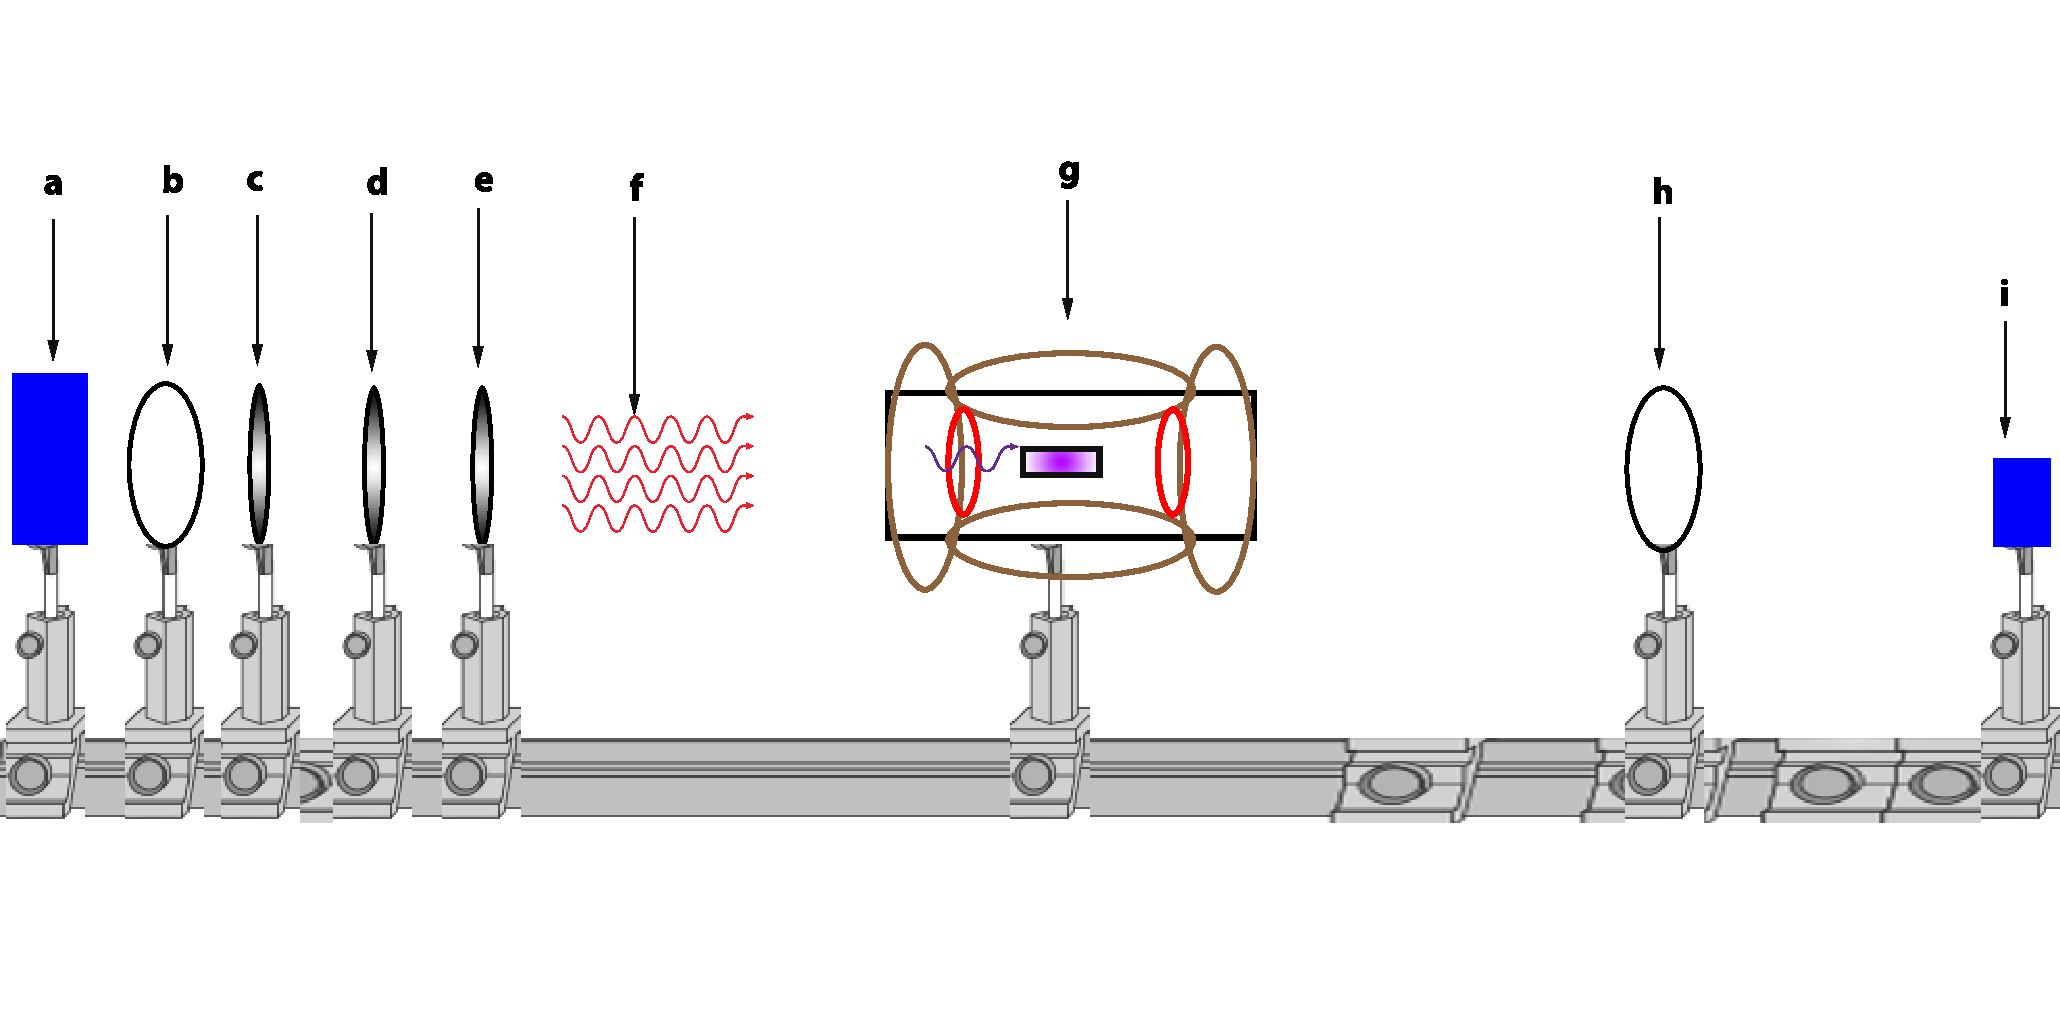
\includegraphics[width=4.7in]{figs/apparatus}
\caption{Leaky faucet experimental apparatus}
\label{apparatus}
\end{center}
\end{figure}

\begin{table}[htp]
\begin{center}
\begin{tabular}{|c|c|}
\hline 
\textbf{Equipment} & \textbf{Manufacturer/Model} \\
\hline 
Weir cup & Central Scientific Company \\
\hline
HeNe Gas Laser & JDSU 1508P-1 633 nm\\
\hline 
Aqua Pump & Rolf C. Hagen Corporation \\
\hline 
Microcontroller & Arduino UNO \\
\hline
Photodiode detector & ThorLabs DET210 \\
\hline 
Oscilloscope Probe & Agilent 10073C \\
\hline 
ND Filter & ThorLabs NE10A \\
\hline 
\end{tabular} 
\caption{Equipment List}
\end{center}
\label{defaulttable}
\end{table}

\newpage
\begin{figure}[htp]
\begin{center}
\includegraphics[width=4.9in]{figs/wiring}
\caption{Close up schematic for Arduino, laser, photodiode detector, ND filter, and oscilloscope probe}
\label{wiring}
\end{center}
\end{figure}

\newpage
%***Coding \newline
\subsection{Coding}
The code for the Arduino can be found in Appendix \ref{App:AppendixA}. As mentioned above, the most important piece of data for us to record is the time of each water drop so we can later determine the period between drops. The code is straightforward but worth going through carefully.

The \texttt{setup()} function on line 5 is run once when the Arduino first turns on. \texttt{Serial.begin(9600)} on line 7 is a function that tells the Arduino we would like to communicate with the Serial output using the 9600 band; this is what lets us interface the Arduino with the computer. Inside the \texttt{setup()} function we also initialize \texttt{time0} to be used later as the initial time to find the period.

The \texttt{loop()} function on line 11 is run over and over again as long as the Arduino is on. Lucky for us, the Arduino keeps track of the number of milliseconds that have passed since it was turned on which we access every time the loop is run with the \texttt{millis()} function on line 13. The Arduino gives us access to the analog voltage value being read on several pins of our choosing (in this case pin A0) using the \texttt{analogRead(pinNumber)} function on line 15. If pin A0 is reading above 500 mV (which it does when the laser is hitting the photodiode detector) then the loop will get skipped, but once the laser beam path is broken the detector will output a lower voltage, which will be read as less than 500 mV by pin A0 and the loop will execute; so it is really on line 15 where we are able to interface between the physical experiment, the Arduino, and the code, which makes line 15 my favorite line.

After stepping into the if-statement on line 15 there is some interesting behavior. Line 16 is where we interface between the Arduino code and Excel. We output the drop number and period to the Serial output; however, we output the data in such a way that it can be imported later into Excel so the data can be processed. Lines 16-17 update the drop number and the initial time to be used when calculating the next period. Finally line 19 addresses the speed at which the Arduino executes an iteration through the \texttt{loop()} function. Because the Arduino is able to run through the \texttt{loop()} function so fast it is possible that the loop will run twice per a single drop, thus it gets counted twice. Because we were measuring periods on the order of 50 ms, a delay of 10 ms, using the \texttt{delay(10)} function, gives a single drop time to make it all the way through the laser while still giving the Arduino time to recover and wait until the next drop, so the double counting problem is solved.

%***Running Experiment \newline
\subsection{Running the experiment}
Surprisingly, displaying useful processed data from the Arduino in real-time is not as easy and one may think. Theoretically, one should be able to send the raw data shown in the top left of Fig. \ref {screen}  to another program such as Matlab or Processing, process the raw data to find the period, and then render a plot such as Fig. \ref{together}. Then one could easily adjust the clamp on the hose shown in Fig. \ref{apparatus} and find different regions of interest and toggle data capture on or off to be used later. In reality, the Arduino software doesn't play nice with other programs except it's own native Serial Monitor which can be seen in the top left of Fig. \ref{screen}. While performing the experiment these numbers are often jumping across the screen and it's hard to get a sense of what type of drip behavior is happening until after the data is processed. After repeating the experiment many times and processing the data it became obvious that most of the interesting behavior was happening somewhere around a period of 50 ms, so this was the region we most closely investigated.

To optimize the possibility of a successful trial run we first pulled a paper towel over the bottom bucket, for the drumming noise. Then we started the Arduino software to begin displaying times for each drop. When the software is running we opened the clamp until we were within range of about 50 ms; this was accomplished by preventing the Serial Monitor from auto-scrolling and checking the output to see if it was on the order of 50 ms. Once we were within range we closed the Serial Monitor and re-opened it to begin the trial. The reason why we close and re-opened the Serial Monitor to begin the trial is the counter starters over again except this time exactly in a region of interest which makes processing the data later much easier. Now a trial run is in full swing and it's time to adjust the clamp to increase or decrease the period and hopefully move into different regions of interest. Now, one may think that using an adiabatic approach by slowly opening or closing the clamp is the way to success; however, in reality when this is done often the region is overshot or hidden because the dropper isn't given a chance to stabilize within a specific region. What ends up happening is the data becomes a swoopy blur and no interesting behavior is observed as shown in Fig. \ref{bad}. The technique we found to be more useful is to instead open or close the clamp as little as possible, but do it quickly and then wait for around 500 drops then make another instantaneous open or close of the clamp. Suffice to say, finding the beautiful display of all three regions in the same trial run, as shown in Fig. \ref{together}, took much effort.

%***processing data \newline
\subsection{Processing data}
One might expect getting measured data out of the Arduino to be easy, especially because the entire community of scientists, hobbyists, students, and anyone performing any type of experiment with the Arduino are likely making some sort of measurement and probably want their data go somewhere besides the Serial Monitor. Actually, finding a way to get data from the Arduino into a usable form like a CSV file in even a pitifully scalable way is non-trivial. We tried several ways including: piping the output to the terminal, piping the output to Processing, piping the output to a file, and crudely copying and pasting the output from the Serial Monitor. Any time another program was being used with the Arduino integrated development environment (IDE) all the programs had to be restarted each time and in a specific order to get reliable results making it impractical for multiple trials. Piping output to a file worked about half the time and only if the entire IDE was shut down in a specific order. Also when trying any of the first three methods mentioned one was not able to open the Serial Monitor first to get an idea of what the current period was and then begin taking data after establishing that we were close to an interesting region. The only reasonable workflow for processing data that allowed us to run many trials and save useable data can be seen in Fig. \ref{screen}: literally copying and pasting data from the Serial Monitor (using cmd-C because the Serial Monitor doesn't respond to right clicks), and then using the ImportText Wizard in Microsoft Excel. However, as shown on the right in Fig. \ref{screen} the Serial Monitor adds it's own newline character to each line so the data ends up skipping every other cell in Excel. To work around this we first copied and pasted the data from the Serial Monitor into Sublime Text, a text editor (keeping in mind to use cmd-A in the Serial Monitor to highlight all the data, otherwise it takes literally 5 minutes of waiting to highlight all the text while the Serial Monitor scrolls), then we copied and pasted the data from Sublime Text into Excel using the ImportText Wizard with Sublime Text automagically (that is, "automatically" but with no explanation for why it works) removed all the mysterious new lines, also shown on the right of Fig. \ref{screen}. Finally we are able to process our data in Excel as one would normally expect.


\newpage
\begin{figure}[htp]
\begin{center}
\includegraphics[width=7in]{figs/screen2}
\caption{ Screen shot of a finished trial and data processing}
\label{screen}
\end{center}
\end{figure}

\newpage
%Data and Analysis
%This section typically includes all of your measurements and/or and raw data in a clearly organized and easy to read format. The `Analysis' part of this section explains how you go from your raw data to a final result. Describe the procedures you used for your calculations.  Some additional theory can be included in this section if it is directly related to your data analysis method.  Show all of your calculations (or in the case of a lot of data, a sample calculation), graphs and any derived numerical results.  

\section{Data, Analysis, and Discussion}
\subsection{Interpreting the graph}
There are three types of graphs that we use to visualize our data. Interpreting each one can take a little getting used to but once understood the information provided by each can be clear. 

\subsubsection{Period vs. drop number}
 Figures \ref{together} - \ref{bad} are plots of period as a function of droplet number. On these types of graphs each point represents a single period between two water droplets. Figure \ref{together} is an experimental plot of the period-1, period-2, and chaotic regions. Figure \ref{together_th} is a theoretical plot of the period-1, period-2, and chaotic regions. Figure \ref{bad} is an experimental plot showing only periodic regions. Taking a look at Fig. \ref{together_th} we can understand what is happening more easily because of the resolution. Notice, how for the period-1 region, also called periodic, droplets 21-30, has the same period of 40 ms. However, when looking at droplets 0-9 we see that for each successive droplet there is a toggling between 50 ms and 70 ms, this behavior is characteristic of period-2, or period doubling. Finally, droplets 10-19 seem to be randomly scattered about, never repeating or alternating, this behavior is characteristic of chaotic dripping.
 
\newpage
\begin{figure}[htp]
\begin{center}
\includegraphics[width=5in]{figs/together}
\caption{ Good data showing Period-1, Period-2, and Chaotic experimental regions}
\label{together}
\end{center}
\end{figure}

\begin{figure}[htp]
\begin{center}
\includegraphics[width=4.6in]{figs/together_th}
\caption{Theoretical Period-1, Period-2, and Chaotic regions with 30 drops}
\label{together_th}
\end{center}
\end{figure}

\newpage
\begin{figure}[htp]
\begin{center}
\includegraphics[width=6in]{figs/bad}
\caption{Adjusting clamp adiabatically, instead of in quick direct bursts produces convoluted data}
\label{bad}
\end{center}
\end{figure}

\newpage
\subsubsection{Poincare section graph}
Figures \ref{periodic_th}, \ref{periodic_exp}, \ref{period_doubling_th}, \ref{period_doubling_exp}, \ref{chaotic_th}, and \ref{chaotic_exp} are Poincare section graphs. Poincare section graphs can be used to zoom in on each region of interest. Now, each point on the graph holds two pieces of information, the period of an initial droplet on the x-axis ($T_n$), and also the period of the next successive droplet on the y-axis ($T_{n+1}$). The line $T_{n+1} = T_n$ represents regions of periodicity because each successive drop has the same period, therefore each successive droplet will map back to the same point.  

Figure \ref{periodic_schematic} shows a visualization of periodic dripping, if we take $n = 1$ then we can see both $T_1$ and $T_2$, in red to signify they have the same period; now when we look at the graph on Fig. \ref{periodic_th} we can see that $T_1 = 40$ ms but $T_2 = 40$ ms also, and so a point on the graph predictably falls onto the $T_{n+1} = T_n$ line.

We can compare the theoretical and experimental Poincare section graphs to determine which region the system is in. Figures \ref{periodic_th} and \ref{periodic_exp} clearly agree indicating that our system is indeed exhibiting periodic behavior.

\newpage
\begin{figure}[htp]
\begin{center}
\includegraphics[width=.9in]{figs/periodic_schematic}
\caption{ Period-1 visualization}
\label{periodic_schematic}
\end{center}
\end{figure}

\begin{figure}[htp]
\begin{center}
\includegraphics[width=4.2in]{figs/periodic_th}
\caption{ Period-1 theoretical plot}
\label{periodic_th}
\end{center}
\end{figure}

\newpage
\begin{figure}[htp]
\begin{center}
\includegraphics[width=6in]{figs/periodic}
\caption{ Period-1 experimental plot}
\label{periodic_exp}
\end{center}
\end{figure}

\newpage
Figure \ref{double_schematic} shows a visualization of period doubling dripping, if we take $n = 1$ then we can see both $T_1$ and $T_3$, in purple to signify they have the same period, while $T_2$ in green to signify it has a different period; now when we look at the graph on Fig. \ref{period_doubling_th} we can see that $T_1 = 50$ ms but $T_2 = 70$ ms, and so a point on the graph falls above the $T_{n+1} = T_n$ line. Now, if we take $n = 2$, then $T_n = T_2$ in green, and $T_{n+1} = T_3$ in purple. Looking back at the graph on Fig. \ref{period_doubling_th} we can see that $T_2 = 70$ ms but $T_3 = 50$ ms, and so a point on the graph falls below the $T_{n+1} = T_n$ line. Interesting with period doubling the data points will falls symmetrically about the $T_{n+1} = T_n$ line.

Comparing the theoretical and experimental Poincare section graphs on Fig. \ref{period_doubling_th} and Fig. \ref{period_doubling_exp} we can see that they clearly agree, indicating that our system is indeed exhibiting period doubling behavior.

\newpage
\begin{figure}[htp]
\begin{center}
\includegraphics[width=.9in]{figs/double_schematic}
\caption{ Period-2 visualization}
\label{double_schematic}
\end{center}
\end{figure}

\begin{figure}[htp]
\begin{center}
\includegraphics[width=3.7in]{figs/period_doubling_th}
\caption{ Period-2 theoretical plot}
\label{period_doubling_th}
\end{center}
\end{figure}


\newpage
\begin{figure}[htp]
\begin{center}
\includegraphics[width=6in]{figs/period_doubling}
\caption{ Period-2 experimental plot}
\label{period_doubling_exp}
\end{center}
\end{figure}

\newpage
Figure \ref{chaotic_schematic} shows a visualization of chaotic dripping, if we take $n = 1$ then we can see both $T_1$, $T_2$, and $T_3$ all have different periods; now when we look at the graph on Fig. \ref{chaotic_th} we can see that there is no predictable pattern and the data points are scattered about the $T_{n+1} = T_n$ line.

Comparing the theoretical and experimental Poincare section graphs on Fig. \ref{chaotic_th} and Fig. \ref{chaotic_exp} we can see that they clearly agree, indicating that our system is indeed exhibiting chaotic behavior.

\newpage
\begin{figure}[htp]
\begin{center}
\includegraphics[width=.7in]{figs/chaotic_schematic}
\caption{ Chaotic visualization}
\label{chaotic_schematic}
\end{center}
\end{figure}

\begin{figure}[htp]
\begin{center}
\includegraphics[width=4in]{figs/chaotic_th}
\caption{ Chaotic theoretical plot}
\label{chaotic_th}
\end{center}
\end{figure}


\newpage
\begin{figure}[htp]
\begin{center}
\includegraphics[width=6in]{figs/chaotic}
\caption{ Chaotic experimental plot}
\label{chaotic_exp}
\end{center}
\end{figure}

\newpage
\subsubsection{Histogram}
We also use a Count vs. Period histogram to zoom in on each region of interest. Now, each bar on the graph tells us how often a specific period occurred for a given number of drops.

Fig. \ref{periodic_hist_th} shows a theoretical histogram for periodic dripping. As expected we see a spike in the 41 to 42 region, which would be the case if the system were in a periodic situation like the one shown in Fig.\ref{periodic_schematic}.

We can compare the theoretical and experimental Histogram graphs to determine which region the system is in. Figures \ref{periodic_hist_th} and \ref{periodic_hist} clearly agree indicating that our system is indeed exhibiting periodic behavior.

\newpage
\begin{figure}[htp]
\begin{center}
\includegraphics[width=4.3in]{figs/periodic_hist_th}
\caption{ Period-1 theoretical histogram }
\label{periodic_hist_th}
\end{center}
\end{figure}
\begin{figure}[htp]
\begin{center}
\includegraphics[width=4.3in]{figs/periodic_hist_2}
\caption{ Period-1 experimental histogram }
\label{periodic_hist}
\end{center}
\end{figure}

\newpage
Fig. \ref{period_doubling_hist_th} shows a theoretical histogram for period doubling dripping. We see two spikes in the 50 to 60 and 70 to 80 regions, which would be the case if the system were in a period doubling situation like the one shown in Fig. \ref{double_schematic}.

Comparing the theoretical and experimental Histogram graphs on Fig. \ref{period_doubling_hist_th} and Fig. \ref{period_doubling_hist} we can see that they clearly agree, indicating that our system is indeed exhibiting period doubling behavior.

\begin{figure}[htp]
\begin{center}
\includegraphics[width=4in]{figs/double_hist_th}
\caption{ Period-2 theoretical histogram}
\label{period_doubling_hist_th}
\end{center}
\end{figure}
\begin{figure}[htp]
\begin{center}
\includegraphics[width=4.4in]{figs/double_hist}
\caption{ Period-2 experimental histogram}
\label{period_doubling_hist}
\end{center}
\end{figure}

\newpage
Fig. \ref{chaotic_hist_th} shows a theoretical histogram for chaotic dripping. We see a wide array of spikes, which would be the case if the system were in a chaotic situation like the one shown in Fig. \ref{chaotic_schematic}.

Comparing the theoretical and experimental Poincare section graphs on Fig. \ref{chaotic_hist_th} and Fig. \ref{chaotic_hist} we can see that they clearly agree, indicating that our system is indeed exhibiting chaotic behavior.

\begin{figure}[htp]
\begin{center}
\includegraphics[width=4in]{figs/chaotic_hist_th}
\caption{ Chaotic theoretical histogram}
\label{chaotic_hist_th}
\end{center}
\end{figure}
\begin{figure}[htp]
\begin{center}
\includegraphics[width=4in]{figs/chaotic_his}
\caption{ Chaotic experimental histogram}
\label{chaotic_hist}
\end{center}
\end{figure}

\newpage


% Discussion
%It is in this section where you discuss your results.  How is your data interpreted?  What features of your data are important and why?  What do your results mean?  How do your results compare with those of the work of others?  Asses whether the results make sense, and explain why.  Error analysis would go in this section.
%\section{Discussion}



\section{Conclusions}

%Conclusion remarks go here.  All results obtained should be concisely summarized here.    
We built an apparatus and wrote custom software to measure the time of each water droplet from a dropper. While building and calibrating our apparatus we solved experimental problems such as decreasing the intensity of the laser to prevent the photodiode from saturating, impedance matching the photodiode detector with the Arduino, using correct technique to attenuate the clamp that adjusts the flow rate, and finding a viable way to process data from the Arduino. By adjusting the flow rate into the dropper, determining the period of each drop, and exploring several different types of data plots we confirmed that our dripping faucet system exhibits periodic, period doubling, and chaotic behavior.

%------------------
%Begin addition of appendix found information at http://tex.stackexchange.com/questions/49643/making-appendix-for-thesis
%------------------
\newpage
\appendix
\section{\\Arduino Code} \label{App:AppendixA}
% the \\ insures the section title is centered below the phrase: AppendixA

\texttt{1 \quad int n = 0;\newline}
\texttt{2 \quad unsigned long time0;\newline}
\texttt{3 \quad unsigned long time1;\newline}
\texttt{4 \newline}
\texttt{5 \quad void setup()\newline}
\texttt{6 \quad \{\newline}
\texttt{7 \quad \quad Serial.begin(9600);\newline}
\texttt{8 \quad \quad time0 = 0;\newline}
\texttt{9 \quad \}\newline}
\texttt{10 \quad \newline}
\texttt{11 \quad void loop()\newline}
\texttt{12 \quad \{\newline}
\texttt{13 \quad \quad time1 = millis();\newline}
\texttt{14 \quad \newline}
\texttt{15 \quad \quad if ( analogRead(A0) $<$ 500 ) \{\newline}
\texttt{16 \quad \quad \quad \quad Serial.println(String(n) + " " + String(time1-time0));\newline}
\texttt{17 \quad \quad \quad \quad n = n + 1;\newline}
\texttt{18 \quad \quad \quad \quad time0 = time1;\newline}
\texttt{19 \quad \quad \quad \quad delay(10);\newline}
\texttt{20 \quad \quad \}\newline}
\texttt{21 \quad \}\newline}

\newpage
\section{\\Appendix B} \label{App:AppendixB}
% the \\ insures the section title is centered below the phrase: Appendix B
\begin{figure}[htp]
\begin{center}
\includegraphics[width=4in]{figs/mushy}
\caption{Successful trial run}
\label{success}
\end{center}
\end{figure}
Infinite thanks to my senior project advisor Dr. Glen Gillen for fun tinkering sessions, reading through long-winded paragraphs, and giving me the equipment and space I needed to work. And another infinite set of thanks to Dr. Matt Moelter for the support and inspiration to see this thing through.
\newpage
%------------------
%End addition of appendix
%------------------

\begin{thebibliography}{99}

\bibitem{shaw}R. Shaw, \textit{The dripping faucet as a model chaotic system},  (Aerial Press, Santa Cruz, USA, 1984.)

\end{thebibliography}

%\appendix

\end{document}


